\chapter{Method and Implementation}

This chapter outlines the work process for this study, designing a methodical approach to investigate emotions in Swedish speech using both AI-based analysis and self-reported data. The chapter describes the study’s approach and design, justifies methodological decisions, provides details regarding data collection and analysis procedures, and addresses validity and reliability considerations. 

\section{Approach and design}
This study adopts an explanatory sequential mixed method approach, which integrates both quantitative and qualitative approaches in a structured sequence. The study first collects and analyzes quantitative data, as AI-generated emotion labels and self-reported emotions, and then qualitative interprets the results to explore alignment and divergence. This approach ensures a systematic, layered analysis rather than pure comparison \autocite{Creswell2023}.  

The study follows a deductive research approach, as it builds upon existing theories of emotional expression in text and speech. The AI models will be tested and compared to established findings. Instead of developing new theories, the study aims to evaluate whether AI-based emotion recognition methods align with each other, prior research on vocal emotion markers and self-reported emotions for Swedish speech. 
This is classified as an experimental study, as it involves a controlled setting where participants are asked questions on predefined emotional recall scenarios. It does not manipulate independent variables in a traditional experimental way \autocite{Creswell2023}, instead observes and analyzes the natural emotional responses provoked through structured questions \autocite{Bryman2022}.

The study evaluates AI-generated emotion labels from speech compared with existing research on vocal markers, text-based emotion recognition and self-reported emotions. The self-reports serve as a reference point and not a ground objective truth, to acknowledge the subjective nature of emotional perception.  

\section{Data Collection}
The study involves participants for semi-structured interviews where they respond to predefined scenarios to provoke emotions. Ethical considerations, such as informed consent and anonymization, are followed firmly to ensure participant well-being. In the first phase, interviews are collected for analysis. 

Approximately 15 Swedish speakers, primarily acquaintances to the researchers, are recruited via invitations. Interviews take place in a quiet room and last for 5-10 minutes including 2-4 scenarios that have been pilot tested for effectiveness, and breaks between the scenarios. Participants complete a self-assessment after each scenario. To minimize acted behavior, the participants are not pre-informed about the feelings that are aimed to be provoked through the scenarios.

Participants are asked open-ended questions designed to bring out previously lived through personal experiences of anger and happiness. The questions about anger are focused on previous experiences of unfair treatment and frustration, while the questions related to happiness explore moments of pride and unexpected joy. The semi-structured format allows for follow-up questions based on participant responses, to bring out as much emotion as possible.
Although there will be a few different predefined scenarios for the participants in the interviews to choose from to maintain freedom in the participants emotional expression, two example questions for both emotions in the interview are:
\begin{itemize}
    \item Can you remember a time when you were treated unfairly by someone? What happened and how did you react?
    \item Tell me about a moment when you were very proud of yourself. What did you do and how did you feel?
\end{itemize}
The study adopts a mixed-method interview approach \autocite{Bryman2022}, where the qualitative data from speech is transformed into quantitative AI-generated emotion labels, to enable comparison in a structured way \autocite{Creswell2023}.
Audio is recorded and analyzed using two emotion recognition models: Hume.ai to extract speech-based emotional labels, and NLP Cloud to transcribe the speech and extract text-based emotional labels. The recordings are preprocessed to reduce background noise. The same dataset is used for all research questions to ensure consistency and all participants remain anonymous.

The diagram in Figure~\ref{fig:pipeline} visualizes the multi-modal pipeline used in this study.  
The interview audio files are processed through three primary channels: speech-to-text transcription via NLP Cloud,  
Speech emotion recognition via Hume AI and acoustic feature extraction via Praat.  
These channels represent two main pipelines.  
The entities presented in yellow are prevalent in both pipelines, where the audio recordings are analyzed with Hume AI, the output is filtered to the 6 emotions analyzed in this study.  
The pipeline illustrated in green represents the analysis to answer research question 1.  
The vocal markers are extracted using Praat Parselmouth.  
The features that are chosen are based on previous research, see \ref{sec:vocal-markers}, Theoretical Framework - Vocal Markers, where pitch, intensity/loudness, formant frequencies (F1, F2, F3), HNR,  
jitter and shimmer have distinguished values for certain emotions.  
To compare the extracted data with Hume AI, these values are clustered into emotion groups.  
Data from speech analysis and vocal markers are combined to statistically analyze the results for RQ1.  
The pipeline used to answer the second and third research question is presented in orange. 
Interview audio is processed the same way as for RQ1 but extended with normalization for the Hume values to enable comparison with outputs from NLP Cloud and self-assessment.  
For text-based emotion recognition, the recording is transcribed before text-analysis is composed. 
Results from speech and text prediction are combined with the self-assessment scores to answer RQ2 and RQ3. 

\begin{figure}[H]
    \centering
    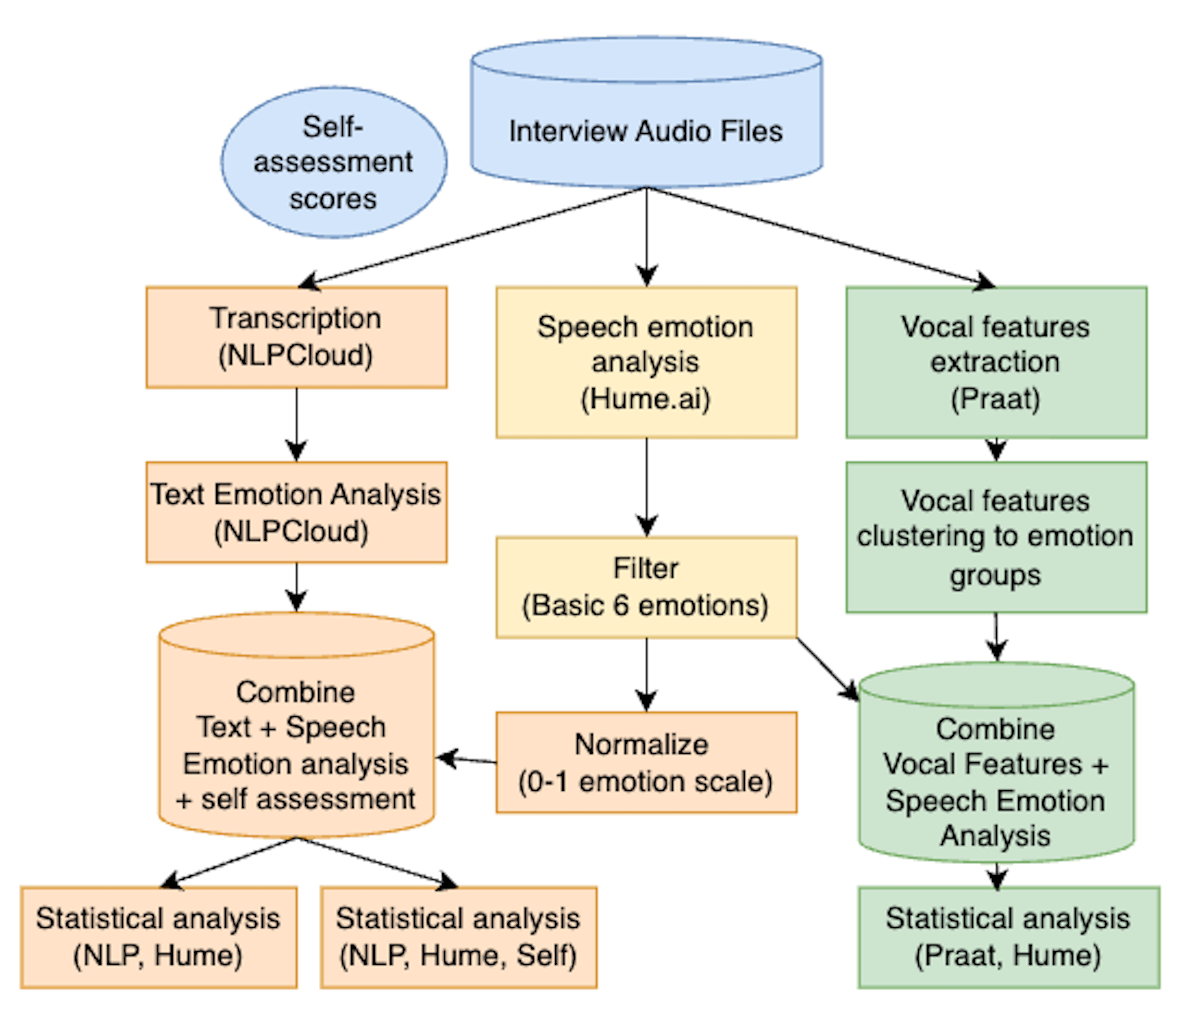
\includegraphics[width=0.8\textwidth]{png/flowchart2.png}
    \caption{The multi-modal pipeline used in this study.}
    \label{fig:pipeline}
\end{figure}


\subsection{Research Question 1}
\textbf{How does AI-model for speech emotion recognition compare to research on vocal markers for emotions in Swedish speech?}

To answer this question, speech recordings are collected from participants as they describe emotionally charged experiences. AI-based emotion recognition using Hume.ai, are used for AI-based Speech Emotion Recognition. Voice feature extraction from the recordings is made, to compare to AI-labeled emotions with known vocal markers from existing Swedish emotion research \autocite{Ekberg2023}. 

\subsection{Research Question 2}
\textbf{Can we understand the emotions from textual content of the speech, with the same data as in RQ1? }

To answer the second question, the recorded speech is transcribed and analyzed for emotion recognition using NLP Cloud’s emotion recognition to assess the emotional content of speech transcripts. The text-based AI labels are compared with speech-based AI labels to determine whether emotion is preserved in textual content alone. 

\subsection{Research Question 3}
\textbf{How do AI-generated emotion labels (speech \& text-based) compare to self-reported emotions? }

For the third question, participants complete a self-assessment survey after each interview segment, where they rate their emotional state on a 1-6 scale (1 = very weak, 6 = very strong) for relevant emotions. The self-reported emotions are compared with AI-generated labels from both speech and text models to analyze agreement and divergence. The results are clustered as agreements, partially agreements, and disagreements across methods. 


\section{Data Analysis}
To evaluate the agreement between different emotion detection methods systematically, diagrams and clustering are used to identify alignment patterns across speech-based AI, text-based AI, and self-reported emotions. The primary goal is to determine if emotion recognition from speech and text aligns with existing research on vocal markers and subjective human perception. If it does not align, the discrepancies will be categorized and analyzed. 

The first step in the analysis involves manual statistical comparison of AI-generated emotion labels with expected vocal markers from Swedish emotion research. This includes alignment degree between speech-based AI emotion labels and known vocal characteristics associated with certain emotions. A high correlation would indicate what the speech-based AI model reflects established vocal emotion markers, while lower correlation suggests potential limitations in the AI’s ability to detect emotions from speech. Additionally, manual clustering is used to categorize cases where the AI model aligns, partially aligns, or diverges from vocal marker expectations.  

The second phase of the analysis assesses the relationship between speech-based and text-based AI models. Diagrams and manual clustering are used for presenting the results, due to the small data set. For cases where the models might diverge strongly, will be analyzed further to identify recurring patterns of misalignment. 

The third stage of analysis focuses on comparing AI-generated labels (speech \& text-based) with self-reported emotions to determine if machine-based emotion detection aligns with human self-perception. Since self-reports are inherently subjective, they are used as a reference point rather than an objective measurement. Correlations are measured to identify tendencies in alignment between AI models and 
self-reports, and to determine whether some emotions show higher agreement than others. 
This will indicate if specific emotions might be easier to recognize regardless of the used method. Manual clustering with diagrams is used to classify responses into full agreement, partial agreement, or divergence. This categorization provides insights about which emotions are most prone to discrepancies between AI models and human perception. 

Comparisons and clustering techniques ensure the study provides a comprehensive evaluation of AI-based emotion recognition and how it correlates to established emotional vocal markers and human perception. Statistical analytic measurements are not used due to the small data set and time frame. The approach allows interpretation of agreement and divergence between different emotion detection methods. 

\section{Validity and Reliability}
\subsection{Validity}
To ensure validity, the interview scenarios are pilot tested to ensure they provoke intended emotions \autocite{Bryman2022}. The use of multiple AI models (speech- and text-based) allows for cross-validation of results. Standardized interview prompts ensure consistency across participants. Participant self-assessment serves as a secondary reference to evaluate AI-labeled emotions. Triangulation across AI, vocal markers, text analysis, and self-assessments enhance convergent validity \autocite{Creswell2023}. 

\subsection{Reliability}
To ensure reliability, standardized equipment and scenario are used to ensure replicability. Hume.ai, NLP Cloud, and Praat provide consistent measures. The AI models used in the study (Hume.ai and NLP Cloud) are pre-trained and validated emotion recognition systems. Correlation will be determined and are used to quantify the reliability of AI models in detecting emotions. The study has a replicable experimental setup, with documentation supporting replication to allow researchers to reproduce similar evaluations.  

Triangulation is achieved in the study through comparison of speech AI, text AI, and self-reports which improves creditability. Any discreteness will be analyzed qualitatively to contextualize potential biases rather than assuming errors. 
Reliability is ensured through standardization in data collection. All interviews are preprocessed to reduce background noise and normalize volume levels. The online tool Auphonic \autocite{Auphonic} is used for this, due to its simple usability for noice reduction, ability to cut out pauses and limit loudness. The same data processing steps are applied consistently for all recordings, ensuring equality in analysis. The study has a replicable experimental setup, with usage of pre-trained, publicly available APIs, and documentation supporting replication to allow researchers to reproduce similar analyses. These measures ensure that our study is generalizable within the scope or automated emotion recognition for stress analysis. 

\section{Considerations}
To consider the implications of this study, several factors must be recognized. To address ethical and privacy concerns, all participant data is anonymized and securely stored to ensure privacy. The participants provide informed consent before engaging in this study. The emotion-provoking scenarios are designed to minimize distress, focusing on natural, everyday emotions rather than triggering events. The participants will have scenarios to choose from, see 2.2 Data Collection. 

Scientific considerations extend to emotion research to Swedish speech and AI tools. Findings in the study can inform future human-interaction research in emotion-based applications. Societal considerations include that the insights could enhance AI-driven mental health tools and future research, especially for Swedish language and real-world interviews. 
